 % -*- root: ../medieninformatik-arbeit.tex -*-
\documentclass[../medieninformatik-arbeit.tex]{subfiles}
\begin{document}
\section{Implementation}
\label{ch:configurator}
The implementation of the activity sculpture configurator and the activity sculpture were undertaken in a period of around two months. The developed web configurator in this work makes use of cutting edge technologies for both web development and 3D visualization. This project is a demonstration of the capabilities of current web technologies that allow the developing of fully functional data visualization systems that offer integration with other web services for data interchange and support real time interactive 3D visualization.

This chapter will discuss all aspects of the technical implementation of the prototypes discussed in chapter \ref{ch:proto}. The technical requirements for the system will be discussed in the first section followed by an overview of the used technologies. Further on the modules conforming the system and their relationship will be explained in the architecture section. THe configurator section covers the implementation of the controls used by the user to manipulate the sculpture and the generation of the sculpture which are the main functionalities covered in the front end side of the application. The integration of the Whithings API and the manipulation performed on the received data are covered in the backend section of the chapter. Finally an overview of the challenges encountered while developing the system is presented. 

\subsection{Requirements}
Through the analysis of current works described in chapter \ref{ch:related},the requirements of the prototypes in chapter \ref{ch:proto} and in view of the forthcoming user study the functionality and technical requirements of the web-based activity sculpture creator were formulated as follows.

\begin{itemize}
	\item Implement the designed configurator workflow views
	\item Users have to be able to login with their personal Withings account
	\item Query user's data with the Withings API
	\item Store user's data and profile information in a data base
	\item Implement user interface control widgets like buttons, sliders and toggles for the customization area of the configurator
	\item Implement the designed activity sculpture geometry
	\item The visualization of the sculpture has to be rendered in real time  
	\item Changes made in the configurator have to be reflected in the sculpture instantly. avoid the use of update buttons 
	\item Users have to be able to navigate the sculpture in 3D space through rotation and zooming interactions
	\item STL file export support for 3D printing
	\item Support for current browsers
	\item Deployment of a fully working version in a web server for the general public. Anybody with a Withings account should be able to use it an visualize their data.
\end{itemize}


The required functionality is beyond what it would be needed for a basic working prototype. The developed configurator in this work is a fully functional system that fulfills every requirement specified in this section. The stated requirements involved the implementation of other functionality to ensure the requirement was fulfilled. For example the login functionality implies the implementation of an Oauth authentication solution(explained later in section \ref{sub:ApiIntegration}) in order to integrate with the Withings API. Also because the configurator is dealing with personal data the security of the system is important, as a basic approach to address this, the configurator implements session handling.

In the following section the used technologies to tackle the extensive list of requirements will be presented.  

\subsection{Technology}
The web configurator was developed with a modern stack of technologies that enable the use of the JavaScript language not only for frontend but also for the backend, the database and graphics programming. The MEAN stack is a collection of technologies that enables developers to write web applications in a single programming language. MEAN is the acronym for the technologies  conforming the stack: \textit{MongoDB}\cite{mongodb}, \textit{Express}\cite{express}, \textit{Angular}\cite{angular} and \textit{Node.js}\cite{joyent2015node}. The acronym was first used by Valeri Karpov, MongoDB engineer, in a blog post\cite{meanstack} where he discussed the benefits of using the same language across all technologies involved. Among the benefits Karpov states their team have experienced an increment in the performance of the developed software and also in the team's productivity.

 MongoDB is a document-oriented database 


 

\textit{Angular Material}\cite{angularmaterial}

Authentication 
\textbf{Passport}\cite{passport} 
\textbf{OAuth} \cite{hammer2010oauth}

Querying user data
\textbf{Withings-API}\cite{withingsApi} 
\textit{RESTful Web services} \cite{Fielding:2000:PDM:337180.337228}
\textbf{WebRTC}\cite{webrtc}
\textbf{SocketIO}\cite{socketio} 

Real time visualization
\textbf{WebGL} \textit{Threejs}\cite{cabello2010three}


\subsection{Architecture}

\begin{figure}[h]
\captionsetup{width=0.8\textwidth}
\begin{center}
  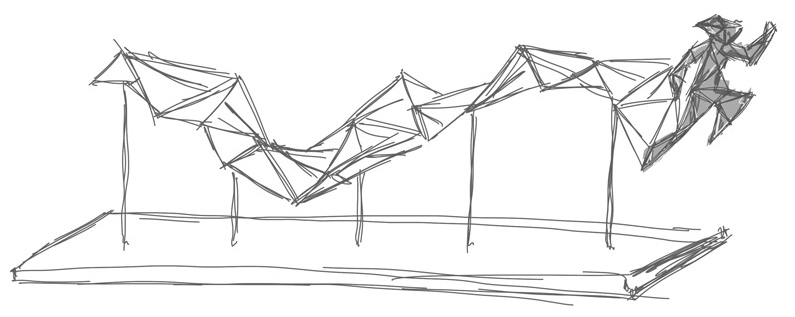
\includegraphics[width=0.8\textwidth]{Prototype/img/3DGraph_detail}
  \caption{Activity Sculpture web configurator's architecture}
\label{fig:architecture}
\end{center}
\end{figure}

\begin{figure}[h]
\captionsetup{width=0.8\textwidth}
\begin{center}
  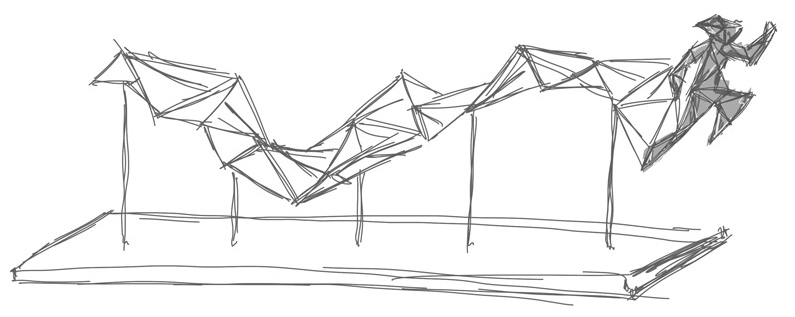
\includegraphics[width=0.8\textwidth]{Prototype/img/3DGraph_detail}
  \caption{Activity Sculpture web configurator's flow diagram}
\label{fig:flowdiagram}
\end{center}
\end{figure}


\subsection{Configurator}
\subsubsection{Sculpture Manipulation}

\begin{lstlisting}[style=htmlcssjs, caption={Example code},label={list:example}]
// create some nodes
var head = document.createElement('h1');
var texto = document.createTextNode("HelloWorld");
// "offline" node manipulation
head.appendChild(texto);
// adding node to DOM
document.getElementsByTagName("body")[0].appendChild(head);
if(!ganas){
	console.log('A wevo a echarle ganas');
}
\end{lstlisting}


\subsubsection{Sculpture Generation \& Rendering}
\label{sub:sculpturegeneration}
\subsection{Backend}
\subsubsection{Withings API Integration}
\label{sub:ApiIntegration}
\subsubsection{Data Processing}
\subsection{Challenges}
\end{document}